%File: formatting-instruction.tex
\documentclass[letterpaper]{article}
\usepackage{aaai}
\usepackage{times}
\usepackage{helvet}
\usepackage{courier}
\usepackage{amsmath}
\usepackage{graphicx}
\usepackage{hyperref}
\usepackage{xcolor}

\frenchspacing
\setlength{\pdfpagewidth}{8.5in}
\setlength{\pdfpageheight}{11in}
\pdfinfo{
/Title (Navigation Project Report)
/Author (Piero Macaluso)}
\setcounter{secnumdepth}{0}
 \begin{document}
% The file aaai.sty is the style file for AAAI Press
% proceedings, working notes, and technical reports.
%
\title{Navigation Project Report}
\author{Piero Macaluso}
\maketitle

\section{Introduction}

The purpose of this document is to briefly present the work done in this project, along with the algorithm used and implemented, but also with a showcase of the results obtained.

This document can be divided into 4 parts:

\begin{itemize}
\item \textbf{Introduction}: the current section;
\item \textbf{Learning Algorithm}: an overview of the approaches and methods used to solve the problem;
\item \textbf{Results}: a presentation of the results reached with plots and GIFs of the best episodes;
\item \textbf{Future Work}: some ideas on how to improve the actual algorithm.
\end{itemize}

\section{Learning Algorithms}

The main starting point of this work was implementing the DQN algorithm \cite{mnih2015human}.
DQN algorithm was the first concrete contact point between Deep Learning and Reinforcement Learning, and it made applying Reinforcement Learning to environments with very large state and/or action spaces possible thanks to the usage of Deep Neural Networks.
In the context of DQN, at each step, based on the current state, the agent chooses an action $\epsilon$-greedily with respect to the action values, and adds a transition $(S_t, A_t, R_{t+1}, \gamma_{t+1}, S_{t+1})$ to a replay memory buffer \cite{lin1992self}, that holds the last transitions. The parameters of the neural network are optimized by using stochastic gradient descent to minimize the loss
\begin{equation}
    R_{t+1} + \gamma_{t+1} \max_{a'}q_\theta^-(S_{t+1}, a') -q_\theta(S_t,A_t))^2
    \label{eq:loss}
\end{equation}
where $t$ is a time step randomly picked from the replay memory. The gradient of the loss is back-propagated only in the \textit{online network} denoted with $\theta$ parameters. Thanks to the usage of experience replay and target networks, DQN is able to learn with stability Q values.

To further explore the concepts, some improvements gathered from the state of the art were analyzed and implemented to improve the performances of the algorithm. The improvements implemented will be briefly presented in this section.

\paragraph{Double DQN}
The vanilla DQN is affected by an overestimation bias caused by the maximization in Equation \ref{eq:loss}. Double Q-Learning \cite{hasselt2010double} addresses this problem by decoupling the selection of the action from its evaluation. In this work, the target network was used to implement this improvement using the loss
\begin{equation*}
    R_{t+1} + \gamma_{t+1} q_\theta^-(S_{t+1}, \arg\max_{a'}(q_\theta(S_{t+1}, a')) -q_\theta(S_t,A_t))^2
    \label{eq:doubleloss}
\end{equation*}

\paragraph{Dueling Networks}

The dueling network \cite{wang2016dueling} is a neural network architecture designed for value based RL. It has a common feature extractor and then two streams of computation, value function and advantage streams. In the approach of this work, they are merged at the end by with the following equation
\begin{equation*}
    \begin{aligned}
    Q(s,a;\theta,\alpha,\beta) = {} & V(s,\theta,\beta){} + \\&(A(s,a;\theta,\alpha) - \frac{1}{|\mathcal{A}|}\sum_{a'}A(s,a';\theta,\alpha))
    \end{aligned}
\end{equation*}

\paragraph{Gradient Clipping}

Gradient Clipping \cite{goodfellow2016deep} clips the size of the gradients to ensure optimization performs more reasonably near sharp areas of the loss surface. It a very simple way to make learning more stable.

\subsection{Hyper-parameters}

The first part of the neural network (the \textit{feature extractor}) is composed of the input layer and one linear layer with a hidden size of 64. After this part, there is the \textit{advantage part} composed of one linear layer with a hidden size of 64 and an output layer with as many outputs as action space size. In parallel, there is the \textit{state value} part which is the same as the previous one, but with an output size equal to one. The network exploits \textit{Rectified Linear Unit} (ReLU) as non-linearity. The hyper-parameters used are presented in Table \ref{table:hp}.

\begin{table}[]
\begin{tabular}{rl}
\textbf{Hyper-parameters}    & \textbf{Value}        \\
Memory Buffer Size          & $10^5$ \\
Batch Size                  & $64$                    \\
Gamma                       & $0.99$                  \\
Tau                         & $10^{-3}$                 \\
Learning Rate               & $5\times 10^{-4}$                  \\
Learning Frequency          & $4$ episodes            \\
Epsilon (start, decay, min) & $(1.0,0.99,0.01)$
\end{tabular}
\caption{Hyper-parameters used in the training process}
\label{table:hp}
\end{table}

\section{Results}

The number of episodes to play was fixed at $1000$, however, the agent took just $365$ episodes to reach an average score on the last 100 episodes greater than $13.0$. The highest average score on the last 100 episodes was equal to $16.56$ reached in $710$ episodes.

The training was not stopped upon reaching the requested value to determine the solution (after $365$ episodes) because it was noticeable that the agent was not so stable. At that stage, the agent frequently got stuck in situations where, while performing complementary actions, he tended to remain stationary in one place as if it were stuck.

To find the best solution, a test phase of 10 episodes was implemented and started every 100 training episodes to evaluate the results without taking into account exploration uncertainties. As shown in Figure \ref{fig:plot}, the best solution was found at episode 1000 \footnote{GIF reporting a handful of seconds of the testing phase \href{https://github.com/pieromacaluso/navigation/blob/daca21c0d0cdcf5bdf7028f7cde85488ea319e50/stuff/test.gif}{\textcolor{blue}{here}}} with an average of $18.60$ over 10 episodes. In this case, blocking situations have become much rarer.

\begin{figure}[]
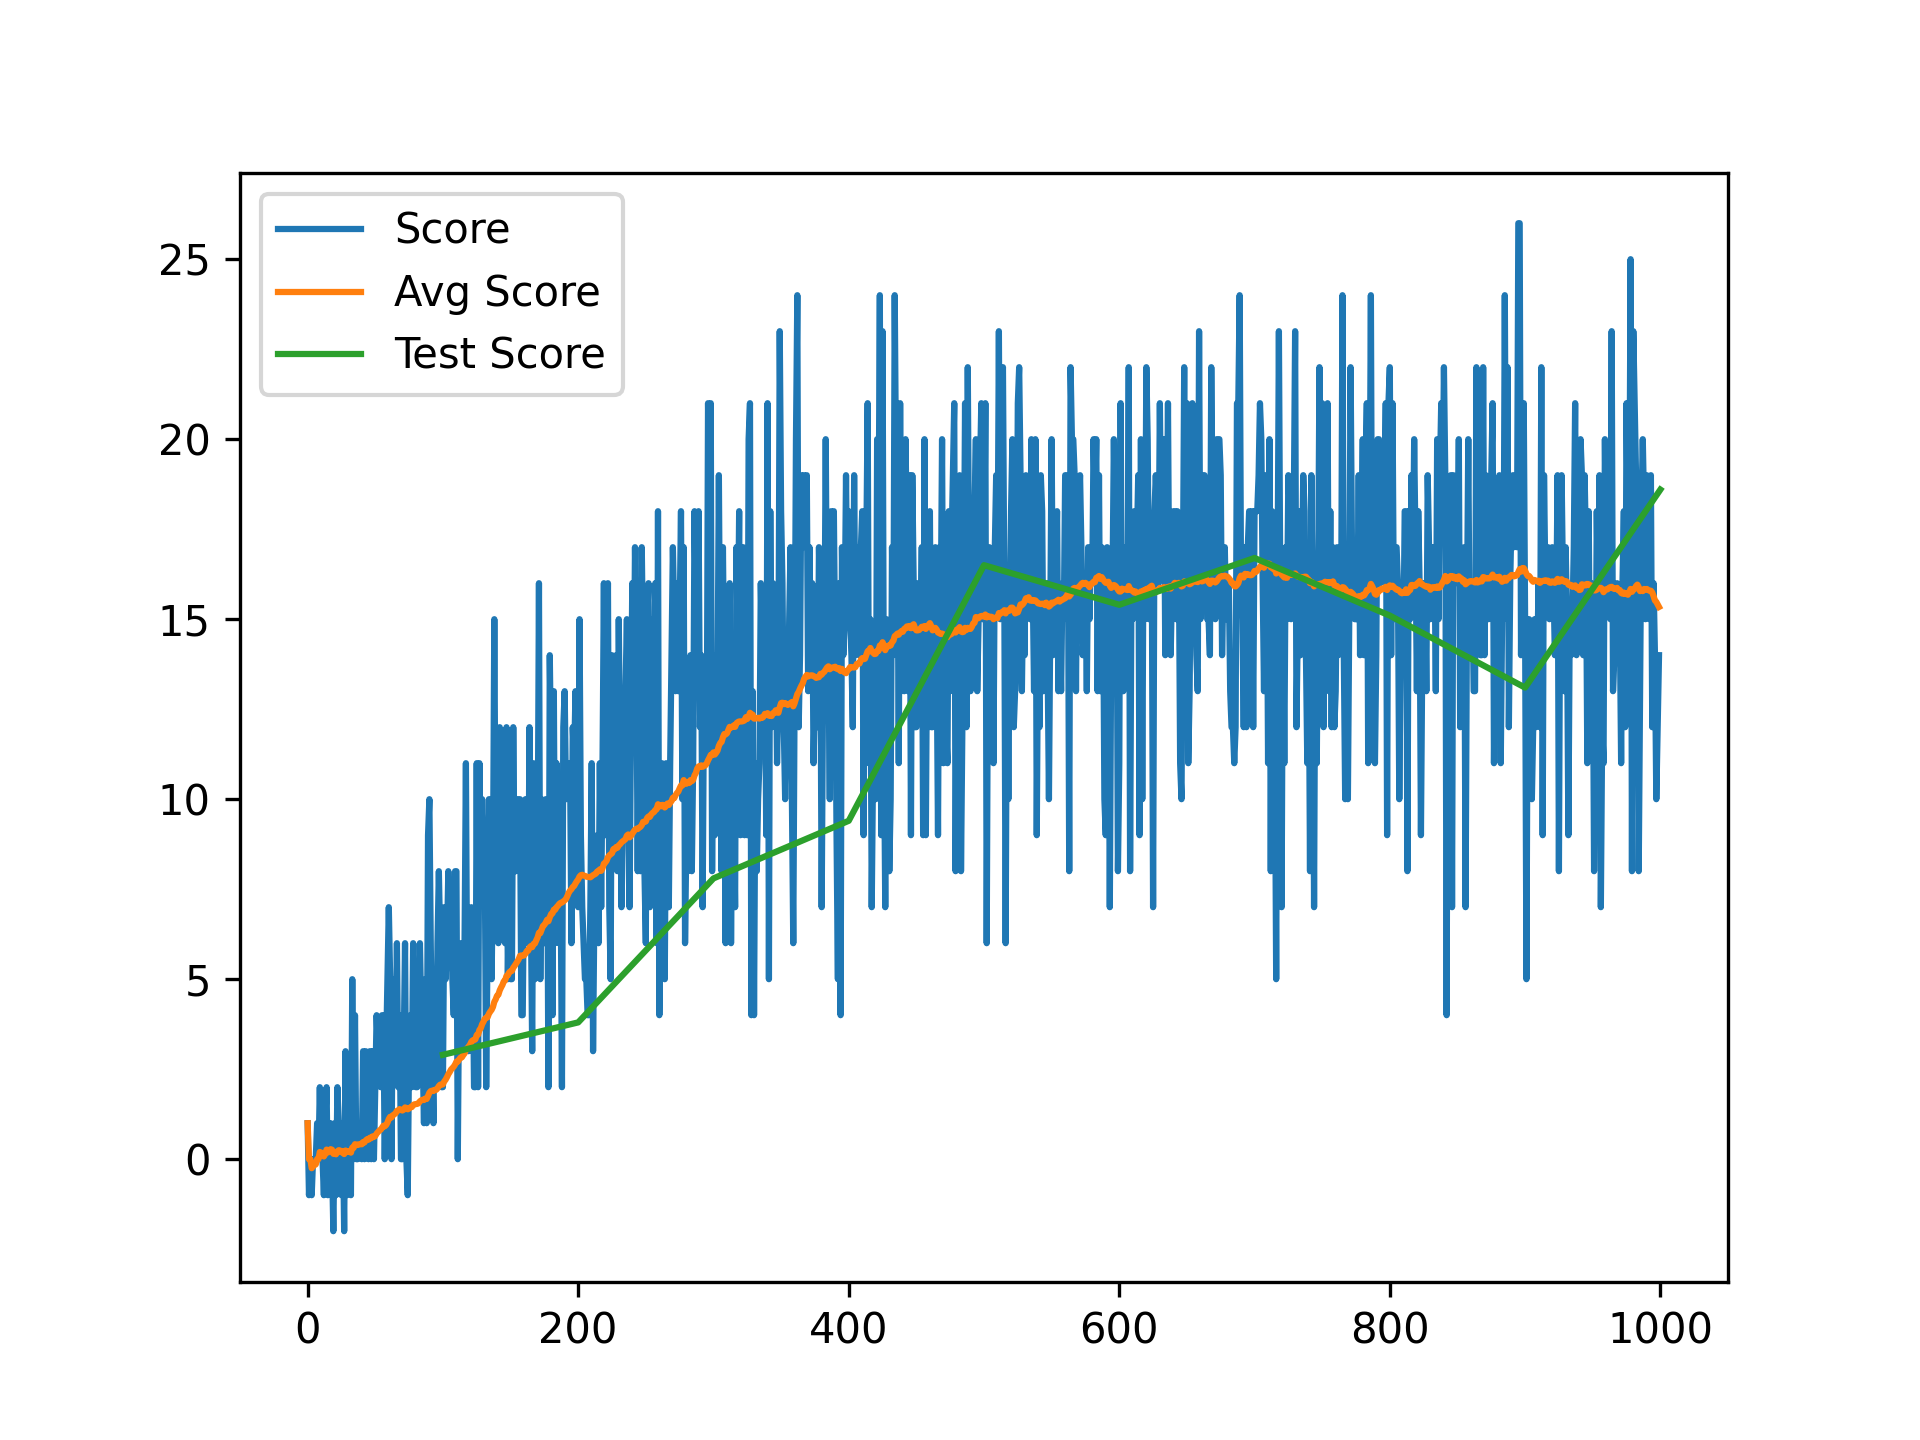
\includegraphics[width=\linewidth]{img/plot_1000.png}
\caption{Training Score History\label{fig:plot}}
\end{figure}   

\section{Future Work}

The results obtained were very encouraging and positive. Despite this, there are a lot of further improvement that is possible to apply to the DQN implemented in this project. Insights about this topic can be found in the Rainbow paper \cite{hessel2018rainbow}, such as Prioritized Experience Memory Replay, Multi-Step Learning, Distributional RL and Noisy Nets to overcome the limitations of $\epsilon$-greedy policies.


\bibliographystyle{aaai}
\bibliography{bibliography}
\end{document}